\section{Analyse de l'existant}
Dans cette partie, nous présenterons les technologies étudiées et leurs qualités. //TOADD//

\subsection{Erco.xyz \cite{Erco}}

Erco est un outil initialement développé à l'Université de Lorraine facilitant la configuration  des routes réseau avec Exabgp en réécrivant une partie du fichier de configuration d'Exabgp. Erco fournit une API RESTful et une interface web utilisateur. L'interface web permet de facilement : annoncer un nouveau réseau ou IP, modifier ou supprimer une route, envoyer des commandes à Exabgp( reload, show routes show neighbors et version).\\
L'esthéthique et les fonctionnalités de cette interface web sont utile pour notre projet. En effet, les bouttons "Relancer Exabgp" et "Exabgp fonctionne" sont exactement ce dont on a besoin. De plus notre section "lancer commande" ressemblera à celui de Erco mais avec plus de commande exécutable et un retour de message de Exabgp plus précis pour chaque commande. Nous prendrons aussi exemple sur Erco pour executer les commandes avec arguments sous forme de formulaire, et afficher les routes sous forme de tableaux, de liste.
Pour essayer la démo en ligne : \url{https://erco.xyz/demo/}
\\
\\
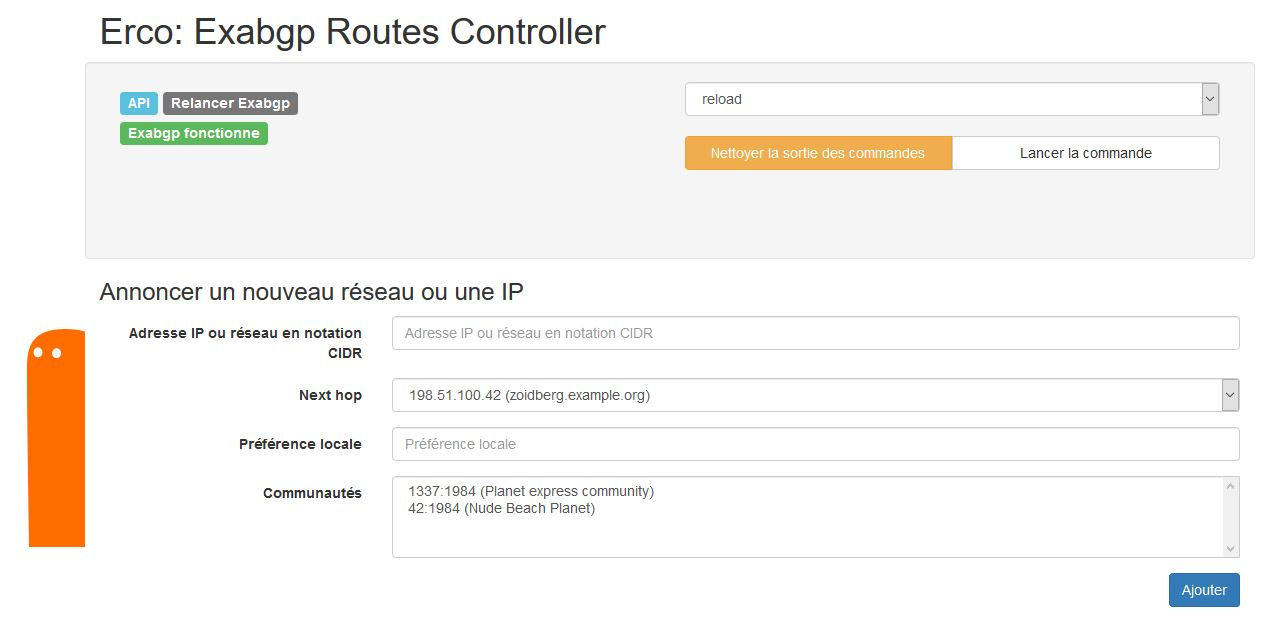
\includegraphics[scale = 0.5]{img/erco1.JPG}
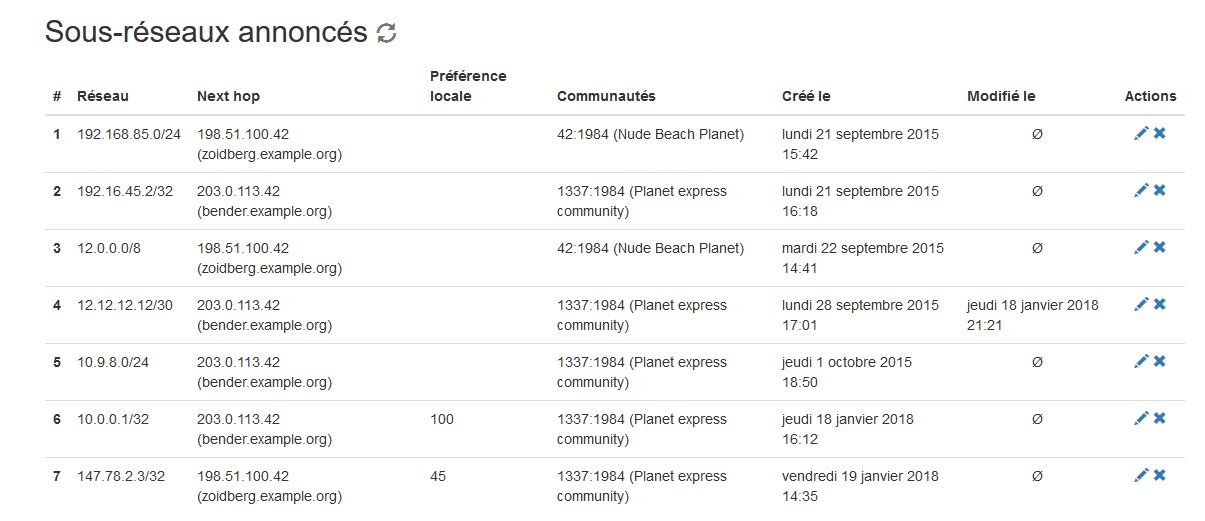
\includegraphics[scale = 0.5]{img/erco2.JPG}

\subsection{ExaBGPmon}
%Faut spécifier pourquoi on veut pas le prendre :
ExaBGPmon est une interface web sur le même principe que Erco.xyz, mais nous n'allons rien retenir de ce site car il est moins intuitif et ergonomique que Erco et propose les mêmes fonctionnalités.
\\
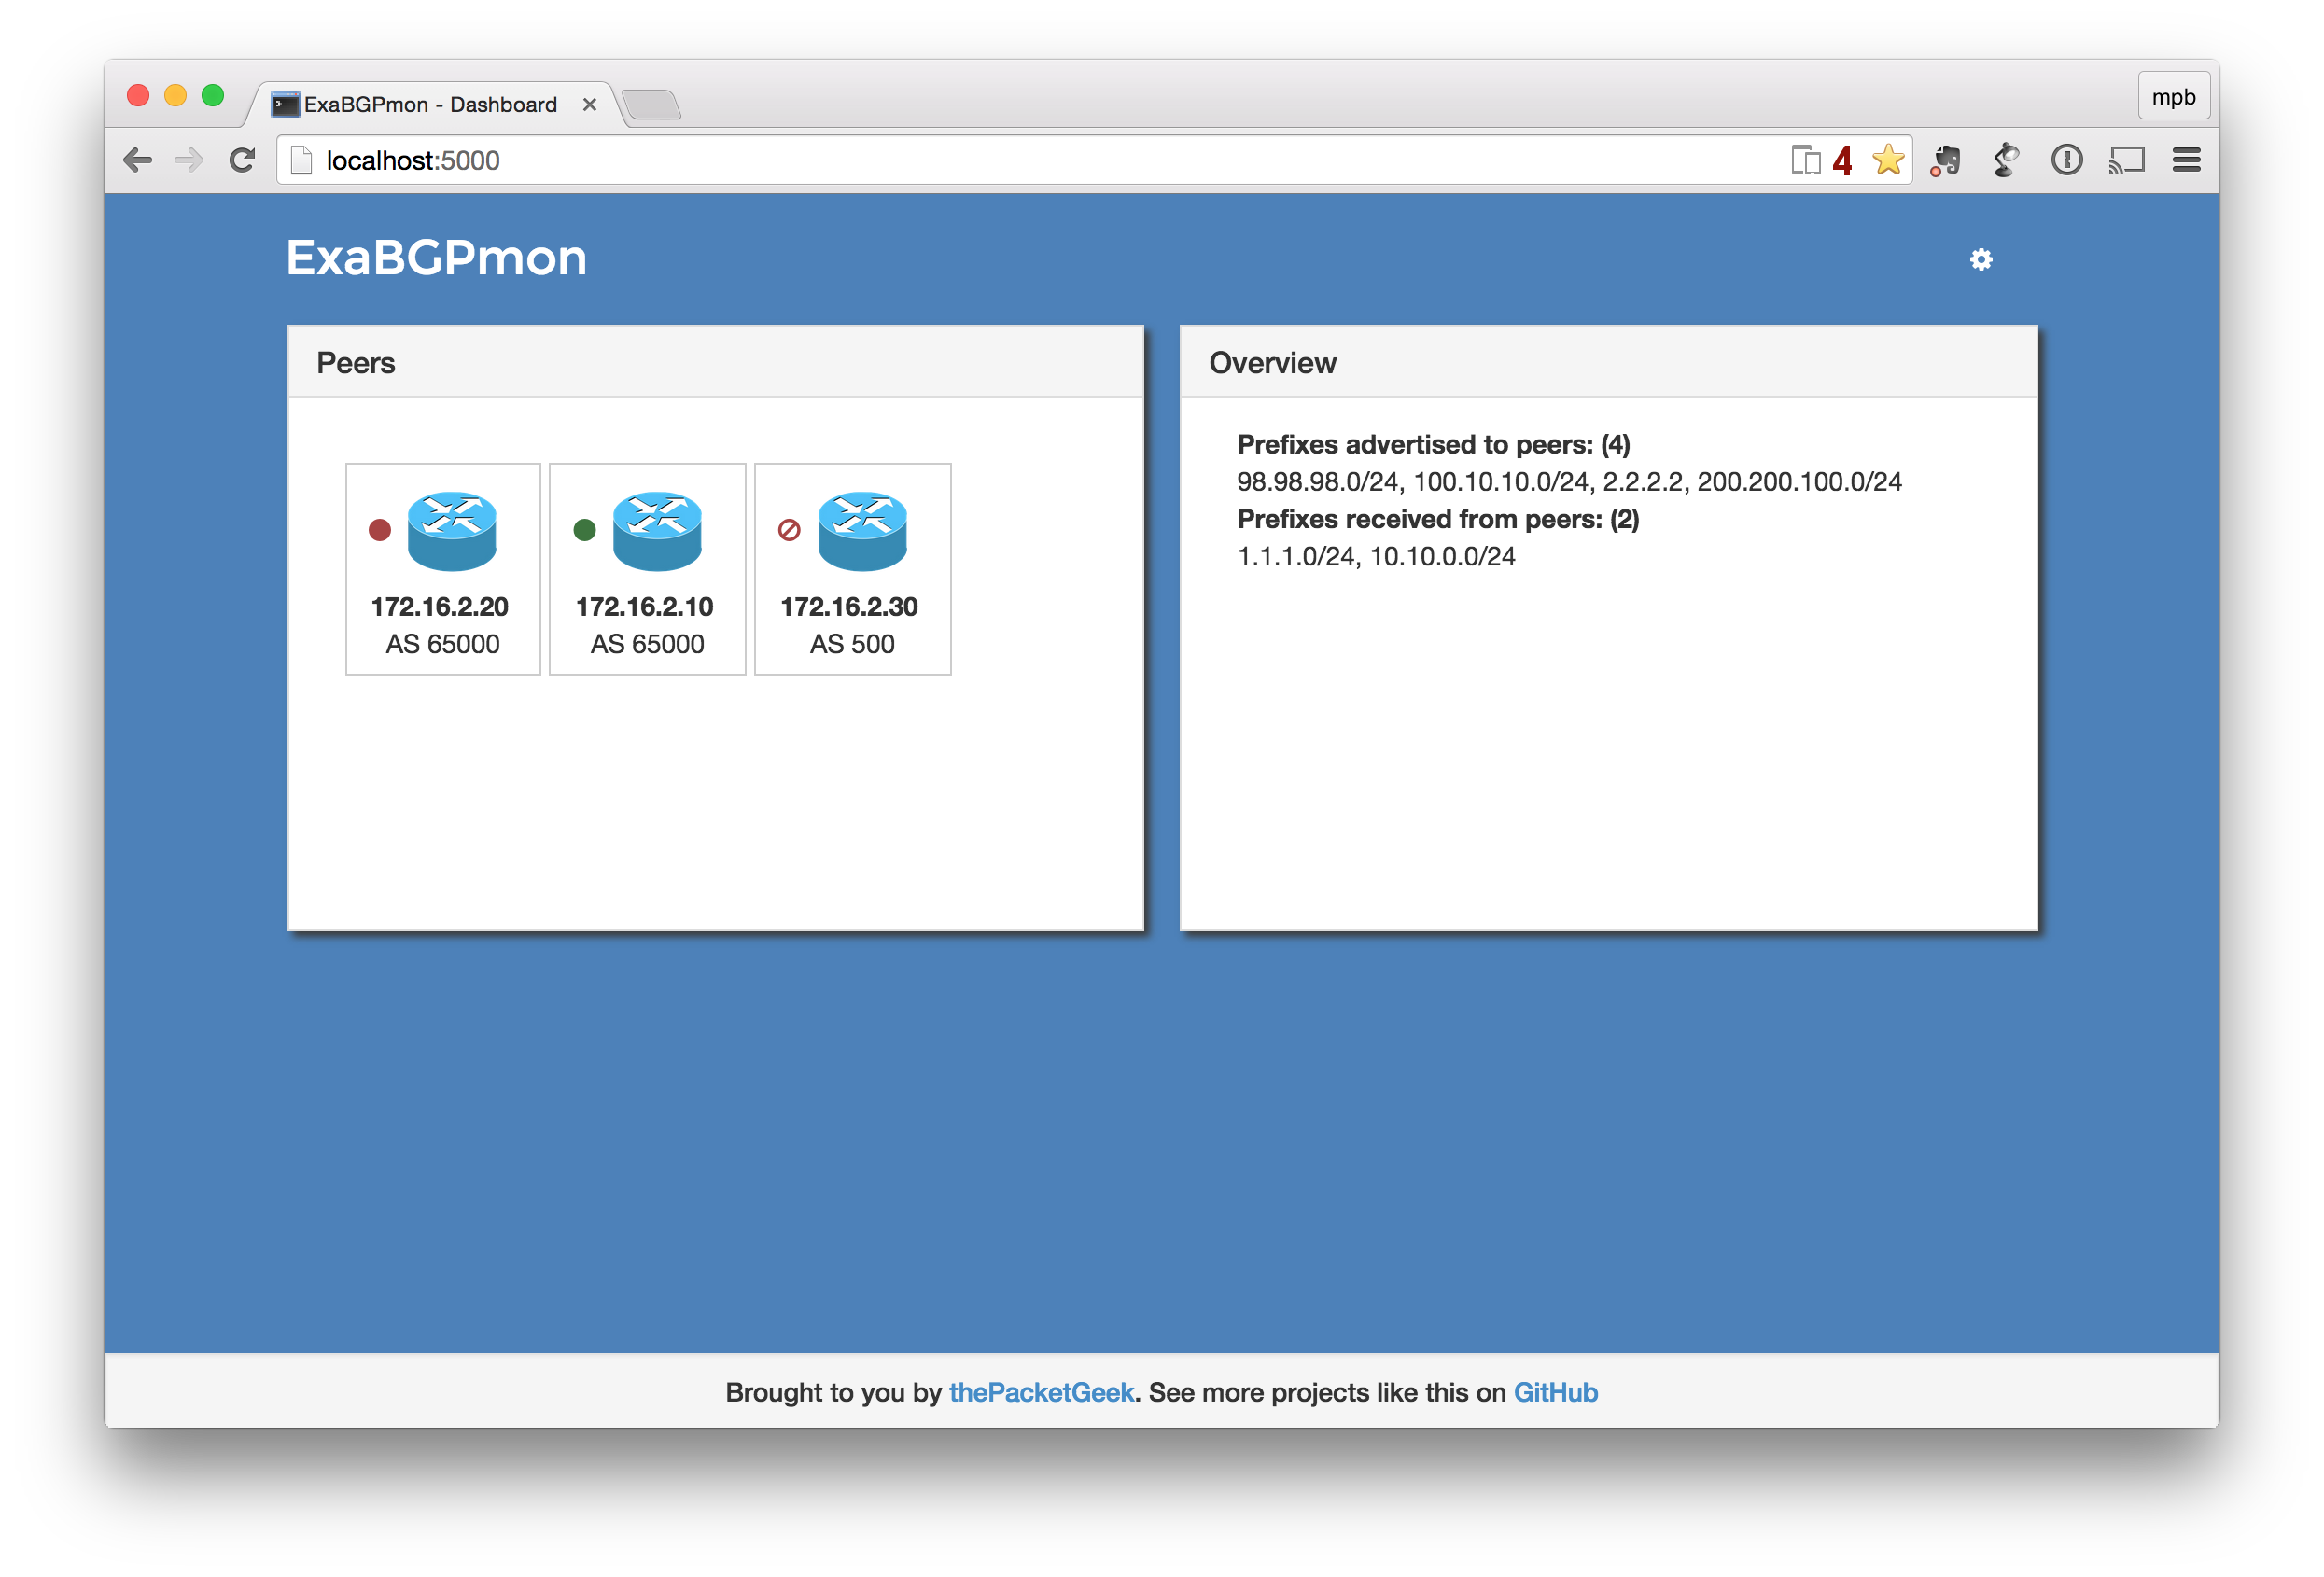
\includegraphics[scale = 0.40]{img/exabgpmon.png}


\subsection{ExaBGP}
ExaBGP est un outil open source écrit en Python qui permet d'interagir avec les réseaux BGP. Le logiciel peut injecter des routes annoncés dans les réseaux, ainsi il permet d'annoncer des routes (configurer des routes).
ExaBGP offre un API contenant plusieurs commandes afin de manipuler les routeurs BGP.
\newline
Notre application Web est censé donc d'envoyer des requêtes HTTP au serveur ExaBGP en Format JSON. Ensuite, ExaBGP prend en entrée le fichier JSON envoyé par notre applciation Web contenant la configuration et les commandes à exécuter par ExaBGP. 
\newline
Enfin, ExaBGP renvoie le message de retour en format JSON pour qu'on puisse le traiter dans l'application Web.
\\
\\
On peut aller voir la liste des commandes dans l'API d'ExaBGP : 
\\
\\
\url{https://github.com/Exa-Networks/exabgp/wiki/Controlling-ExaBGP-:-interacting-from-the-API}
\\
\\
Et apprendre à l'utiliser avec les tutos suivants:
\\
\\
\url{https://thepacketgeek.com/series/influence-routing-decisions-with-python-and-exabgp/}

\subsection{Meteor.JS \cite{Meteor.JS}}
\begin{center}

\includegraphics[height=1cm]{img/Meteor-logo.png}
\end{center}

Meteor.JS est un framework open-source javascript, Node.JS qui permet l'élaboration d'une application web de type RESTful. Elle permet de développer le client et le serveur de l'application web avec le même langage.\\
Notre client voulait une interface web développé en JavaScript de type Restful. Pour un déploiement et implémentation plus rapide de cette interface nous avons décidé d'utiliser le framework open-source Meteor.js qui réponds à ses besoins. De plus avec la possibilité d'utiliser des packages (extensions) de meteor.js nous pouvons implémenter certaines choses plus rapidement.\\
\\
Les packages utilisés sont:
%faut détailler plus pour les packages
\begin{itemize}
\item twbs:bootstrap
\item ian:accounts-ui-boostrap-3
\item iron:router
\end{itemize}

%client javascript RESTfull, nous plus facile package, serveur cache client.
\vspace{0.5cm}
Voici quelques liens pour pouvoir s'informer plus sur Meteor.js:
\\
\\
\url{http://meteortips.com/first-meteor-tutorial/}\\
\url{http://meteortips.com/second-meteor-tutorial/}\\
\url{http://www.meteor-tuts.com/}\\
\url{https://www.meteor.com/tutorials/react/creating-an-app}\\
Documentation: \url{http://docs.meteor.com/#/full/}


\subsection{MongoDB \cite{MongoDB}}

MongoDB est une base de données NoSQL open source orientée documents qui fournit de hautes performances, une haute disponibilité, et mise à l'échelle automatique. L'API MongoDB est compatible avec Meteor.
Les données manipulées sont structurées au format BSON (pour "Binary JSON" lui même acronyme de "JavaScript Object Notation"). Un tel document est une structure de donnée composée de paires champs/valeur. Les valeurs de ces champs peuvent être d'autres documents, des tableaux, ou des tableaux de documents.


Lien de la documentation avec tuto: \url{https://docs.mongodb.com/}

Lien d'un tuto de la documentation de Meteor détaillant la gestion des données avec MongoDB: \url{https://docs.meteor.com/api/collections.html}

\subsection{Dynamips}
Dynamips est un émulateur de routeurs Cisco écrit par Christophe Fillot. Dynamips peut émuler plusieurs versions de routeur Cisco, ainsi il peut lancer différentes images OS Cisco. Dans le contexte de ce projet, on utilise l'image '7200'.

Afin d'installer Dynamips, on aura besoin d'installer certaines bibliothèques :  "libpcap", ou "winpcap" en fonction du système. ces bibliothèques sont utilisées pour fournir les fonctionnalités de "bridging router interfaces" utilisés par les cartes réseaux physiques.
\newline
Ensuite, il suffit de télécharger Dynamips depuis GitHub : 
\begin{center}
\url{https://github.com/GNS3/dynamips}
\end{center}

Afin d'optimiser et de configurer Dynamips, on peut également utiliser  Dynagen.
\newline
Dynagen est un outil écrit en python permettant de paramétrer le fonctionnement de Dynamips en se basant sur des fichiers textes. De plus,  Dynagen simplifie le lancement et la configuration de réseaux virtuels. Cependant, nous n'envisageons pas de l'utiliser dans un premier temps.
En effet, il ne nous sera utile que dans un but d'optimisation des performances. 

\pagebreak

\subsection{NEMU}
NEmu(Network Emulator for Mobile Universes) est un environnement de réseaux virtuels distribués. NEmu gère un parc de machines virtuelle QEMU(un émulateur de matériel \footnote{site officiel: \url{https://www.qemu.org/index.html}}) hébergé sur un ou plusieurs hôtes physiques afin de construire une topologie virtuelle. 

Nemu fournit un interpréteur python afin de créer facilement des réseaux virtuels distribués.
En ce qui nous concerne, on va utiliser cet outil pour pouvoir créer et virtualiser des topologies virtuelles. Alors pour installer Nemu sur linux, on suit les instructions décrites dans ce lien : 
 \url{http://nemu.valab.net/index.php?static27/tuto-setup-nemu-linux}.
 \\
 Concernant la documentation de Nemu, on peut également la trouver dans le lien suivant : 
 \begin{center}
 \url{http://nemu.valab.net/index.php?static2/doc}
 \end{center}